\documentclass{beamer}
\usetheme{Darmstadt}
\usecolortheme{beaver}
\usepackage{booktabs}

\usepackage[utf8]{inputenc}
\usepackage{graphicx}
\graphicspath{ {./images/} }


%Information to be included in the title page:
\title{Homework 1 Presentation}
\author{Brandon Hosley}
\institute{University of Illinois - Springfield}
\date{\today}

\begin{document}
\frame{\titlepage}

\begin{frame}{Overview}
\tableofcontents
\end{frame}

\section{Supervised and Unsupervised Learning}
\begin{frame}{Supervised and Unsupervised Learning}
\begin{itemize}[<+->]
	\item[Q:] What's the difference between Supervised and Unsupervised learning? \\
	\item[A:] Training data is \emph{well} labeled, with \emph{ground truth}.
\end{itemize}
\end{frame}

\begin{frame}{Supervised and Unsupervised Learning}
\twocolumn[]
\end{frame}

\begin{frame}{For Example:}
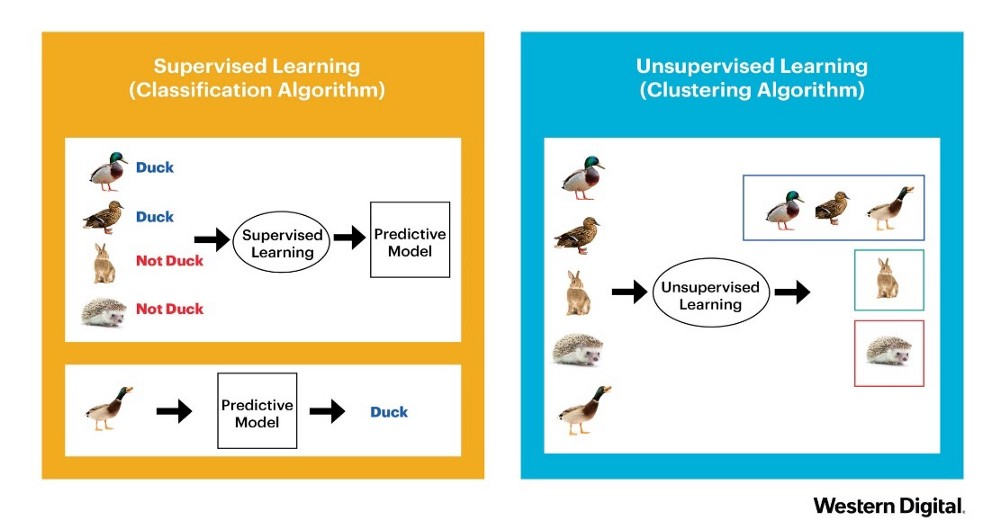
\includegraphics[width=\linewidth]{SupVsUnsup}
\end{frame}


\section{Hastie and Tibshirani}

\begin{frame}{Hastie and Tibshirani}

\end{frame}

%%%%%%%%%%%%%%%%%%%%%%%%%%%%%%%%%%
\begin{frame}
\frametitle{Sample frame title}
\begin{block}{Remark}
	Sample text
\end{block}

\begin{alertblock}{Important theorem}
	Sample text in red box
\end{alertblock}

\begin{examples}
	Sample text in green box. The title of the block is ``Examples".
\end{examples}

\end{frame}

\end{document}
